\documentclass[11pt]{beamer}
\usetheme{Warsaw}
\usepackage[utf8]{inputenc}
\usepackage{amsmath}
\usepackage{amsfonts}
\usepackage{amssymb}
\usepackage{color}
\usepackage{siunitx}


\usepackage{tikz}
\usetikzlibrary{shapes,snakes,arrows,positioning}


% Define box and box title style
\tikzstyle{mybox} = [draw=red, fill=blue!20, very thick,
    rectangle, rounded corners, inner sep=10pt, inner ysep=20pt]
\tikzstyle{fancytitle} =[fill=red, text=white]

\author{Arindam Basu}
\title{Vacuum Measurement}
%\setbeamercovered{transparent} 
%\setbeamertemplate{navigation symbols}{} 
%\logo{} 
\institute{IADD, BARC} 
%\date{} 
%\subject{} 
\begin{document}

\begin{frame}
\titlepage
\end{frame}

%\begin{frame}
%\tableofcontents
%\end{frame}




\begin{frame}{Plan of Talk}

\begin{block}

	\begin{itemize}
		\item Introduction
		\item  Classification of vacuum and measurement.
		\item  Various type of gauges and their operating principle
		\item  Gauge care
		\item  Selection of a gauge
		\item Conclusion
	\end{itemize}

\end{block}



\end{frame}


\begin{frame}{Scientific Measurement}

     \begin{center}
		\includegraphics[width=0.3\textwidth]{Gallileo.jpeg}
		\end{center}
     
     ``Measure what can be measured, and make measurable what cannot be measured."  Galileo Galilei

\end{frame}




\begin{frame}{Definition of Vacuum}

\begin{block}

	\begin{itemize}
		\item  Vacuum is the condition in a closed volume where pressure is \textbf{less} than the normal atmospheric pressure. 
		\item  To classify and measure the vacuum, it is very important to define the normal atmospheric pressure.
		\item  At  $0^{0}$  C or 273 K, atmospheric pressure is equal to the weight per unit area of  760 mm column of mercury.
		\item  In vacuum terminology 760 mm column of mercury is known as \alert{760 Torr}, in honour of Italian scientist Torricelli who first created vacuum. Thus 1 mm  of mercury column is equal to 1 Torr.
		
	\end{itemize}

\end{block}



\end{frame}

\begin{frame}{Classification of Vacuum}
Vacuum can be classified in four broader categories. These are 
\begin{center}
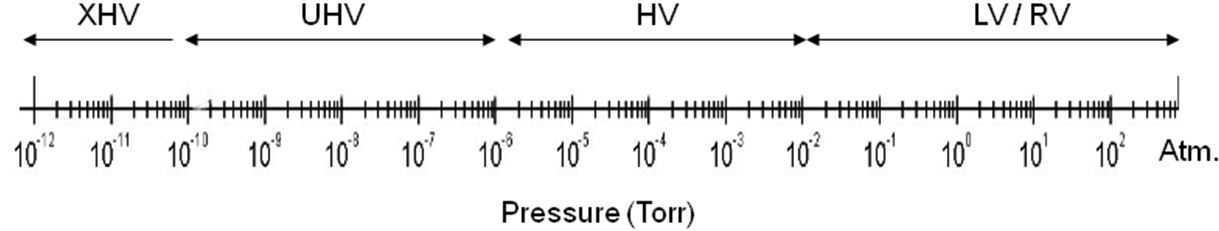
\includegraphics[width=1.0\textwidth]{Vacuum_Scale.png}
\end{center}

\begin{block}{}
\begin{itemize}
\item  Rough Vacuum 	:  $759$ to $1x 10^{-3}$ Torr
\item  High Vacuum   	:  $1x 10^{-3}$ Torr to $1x 10^{-6}$  Torr
\item  Ultrahigh Vacuum  :$1x 10^{-6}$  Torr to $1x 10^{-10}$ Torr
\item  Extra High Vacuum : Less than $1x 10^{-10}$ Torr
\end{itemize}
\end{block}


\end{frame}

\begin{frame}{Units of Vacuum}


     As vacuum is a state of lower gas pressure so unit of pressure such as Pascal or bar can be used to measure and describe the vacuum. \\
     Though occasionally vacuum is expressed in terms of Pascal or bar but there is a unit defined to express the vacuum only. \\
     Most frequently used unit in vacuum is Torr and milli bar(mbar).\\
     
		\begin{center}
		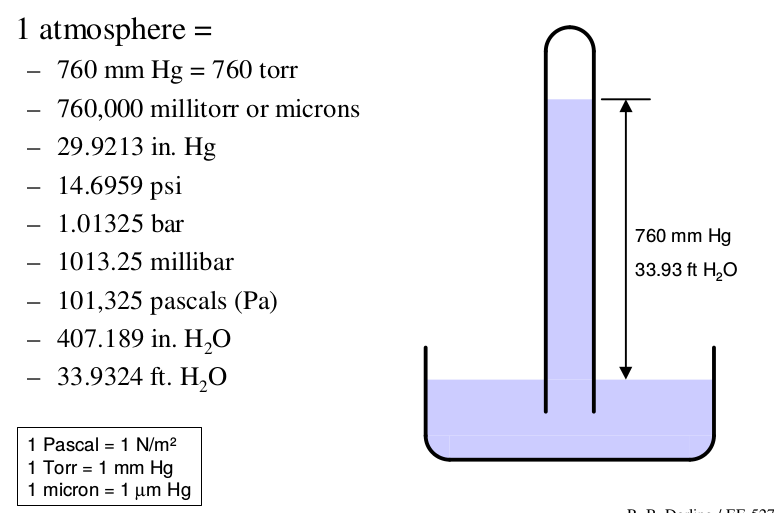
\includegraphics[width=0.7\textwidth]{VacuumUnit.png}
		\end{center}


\end{frame}


\begin{frame}{Vacuum Measurement}


\begin{itemize}
\item Vacuum Measurement is nothing but measuring pressure less the normal atmospheric pressure
\item The atmospheric air is composed of various gases in certain fix proportion and each gas exerts force, the force per unit area is Pressure. 
\item \textbf{Vacuum Gauge} is a piece of equipment used to measure the vacuum inside a closed container.

\item A single gauge can’t measure vacuum starting from atmosphere ($\approx 10^3 $ Torr) to extra high vacuum ($ < 10^{-12} $ Torr) , a span of 15 order or more. Hence this entire range is broken in smaller ranges and most suitable gauges are used in each range. Each range is having one or more suitable gauges and according to requirement/situation gauges are chosen.
\end{itemize}







\end{frame}


\begin{frame}{Gauge Classification}
Vacuum Gauge is a device which measures vacuum of a closed volume. It generally consists of a sensor , control unit and display unit. In this talk we will talk mainly about sensor part.
\begin{center}
\includegraphics[width=0.75\textwidth]{GaugeClassification.pdf}
\end{center}

\end{frame}



\begin{frame}{Uses of Vacuum Gauge}

	\begin{block}{Uses of Vacuum Gauge}

	   \begin{itemize}
          
           \item Vacuum Measurement.
            
            \item Degassing rate estimation.
            
            \item Finding out nature of the leak.	      
	      
	    \end{itemize}
	
	
	\end{block}

\end{frame}





\begin{frame}{Gauges used in the different ranges}

\begin{exampleblock}{Gauges used in high pressure to slight vacuum}

	\begin{enumerate}
	
	
		\item Bourdon Tube
		\item Capacitance Manometer
		\item U Tube Manometer
		 
		
	\end{enumerate}

\end{exampleblock}

\begin{exampleblock}{Gauges used in rough vacuum range}

	\begin{enumerate}
	
		\item  Thermocouple Gauge
		\item  Pirani Gauge
		\item  Manometer Gauge
		
	\end{enumerate}

\end{exampleblock}




\end{frame}



\begin{frame}{Gauges used in the different ranges(contd.)}

\begin{exampleblock}{Medium Vacuum($10^{-3}$  to $10^{-6}$  Torr) }

	\begin{enumerate}
	
		\item Pirani Gauge
		\item Cold Cathode (Penning) Gauge
		 	
	\end{enumerate}

\end{exampleblock}

\begin{exampleblock}{High Vacuum($10^{-6}$  to $10^{-8}$   Torr)}

	\begin{enumerate}
	
	
		\item Cold Cathode Ionisation Gauge Penning Gauge
		\begin{enumerate}
		\item Magnetron Gauge
		\item Inverted Magnetron Gauge
		\end{enumerate}
		\item  Hot Cathode Ionisation Gauge
		\item  Mass Spectrometer(RGA)
			
	\end{enumerate}

\end{exampleblock}

\begin{exampleblock}{Calibration Gauge}

	\begin{enumerate}
	
	
		\item Macleod Gauge
		\item Spinning Rotor Gauge.
			
	\end{enumerate}

\end{exampleblock}



\end{frame}


\begin{frame}{Measurement of Atmospheric Presure}

    
     
     \begin{columns}[t]
    
      
   \column{0.5\textwidth}
       \begin{exampleblock}{}
          \begin{center}
			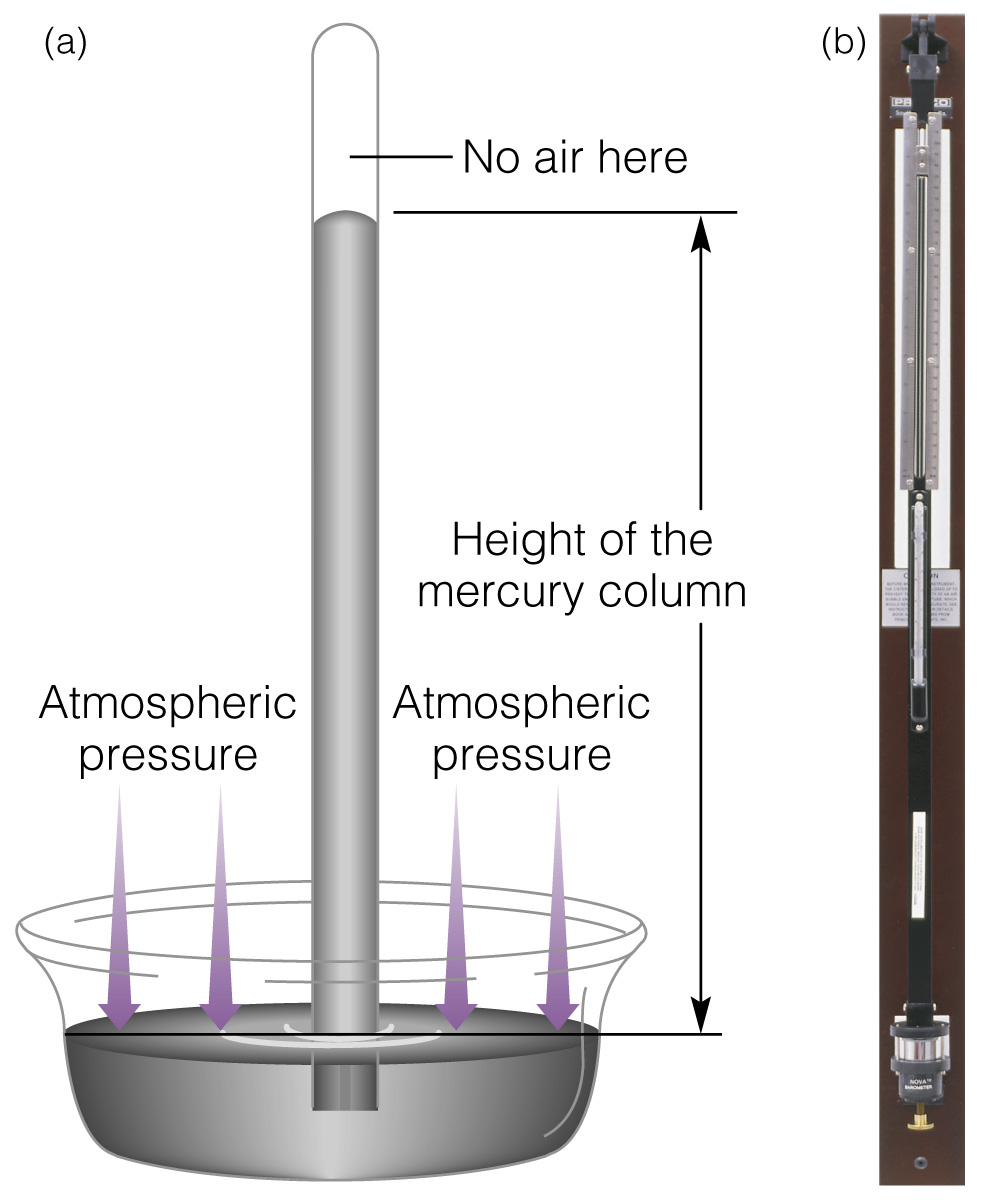
\includegraphics[width=0.9\textwidth]{barometer.jpg}
		\end{center}
       \end{exampleblock}
       
    \column{0.5\textwidth}
       \begin{exampleblock}{ }
          
            \begin{itemize}
            	\item Barometer measures the total atmospheric pressure in terms of liquid column height. 
                \item  The liquid can be water, mercury or low vapour pressure oil.
                \item  Other methods of vacuum measurement use some physical property of gas eg. temperature, resistance, air friction etc.
            \end{itemize}
            
         
       \end{exampleblock}   
   
    \end{columns}   

\end{frame}





\begin{frame}{Bourdon Tube}

\begin{columns}[t]
    
      
   \column{0.4\textwidth}
       \begin{exampleblock}{}
          \begin{center}
			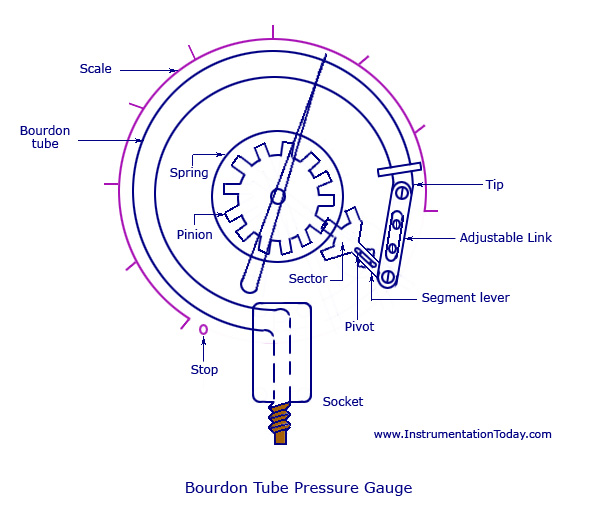
\includegraphics[width=0.9\textwidth]{Bourdon-Tube-Pressure-Gauge.jpg}
		\end{center}
       \end{exampleblock}
       
    \column{0.6\textwidth}
       \begin{exampleblock}{ Features }
          
           \begin{itemize}
           		\item  Rugged and reliable
           		\item Measures relative pressure i.e. Gauge pressure.
    					(Gauge pressure is the pressure relative to the local atmospheric or ambient pressure)
    			\item Suitable for pressure measurement above and below atmosphere.
  		 \item  Can measure pressure in the range 1500 kg/cm2  to vacuum around 1.0 to 0.1 Torr.
           \end{itemize}
   
         
       
       \end{exampleblock}   
   
    \end{columns}   

\end{frame}



\begin{frame}{Bourdon Tube-Construction and Working}

      \begin{center}
			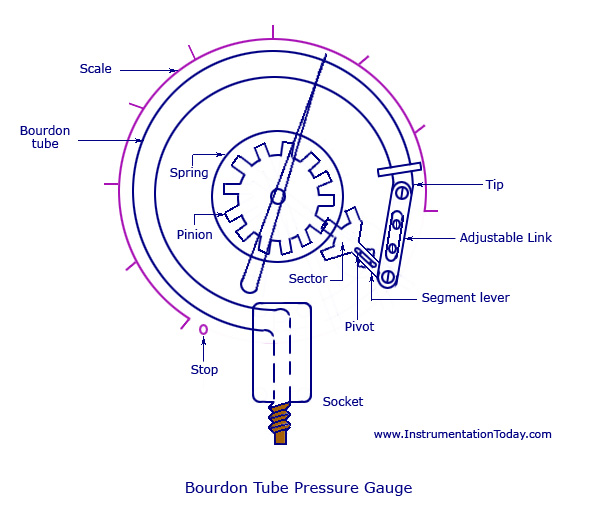
\includegraphics[width=0.4\textwidth]{Bourdon-Tube-Pressure-Gauge.jpg}
		\end{center}
      
       \begin{exampleblock}{Constructional Feature}
          \begin{itemize}
           
           \item The pressure measuring element is a bent elliptical tube. In some special cases Diaphragm, Spring or  Helix are also used.
           \item The tube material could be Phosphor Bronze, Brass, Monel, Beryllium – copper alloy or even Stainless Steel. 
           \item Non metallic elements like neoprene leather is also used in some special cases.
           
           %\item Calibration done by comparing pressure readings with a standard Gauge.
          \end{itemize}
        
       
       \end{exampleblock}


\end{frame}

\begin{frame}{Bourdon Tube-Advantage Limitation and Application}

       \begin{exampleblock}{Advantages}
          \begin{itemize}
           
           \item Portable
 
           \item Convenient to Use
           
           \item No Leveling is required.
           
                     
          
          \end{itemize}
        
       
       \end{exampleblock}
       
       \begin{exampleblock}{Limitations}
          \begin{itemize}
           
           \item Can measure static or quasi static pressure.
 
           \item Accuracy is less. Not suitable for very precise measurement requirement.
           
          \end{itemize}
        
       \end{exampleblock}


        \begin{exampleblock}{Applications}
           Suitable for pressure measurement of furnace draft, pump head, air duct etc.   
        \end{exampleblock}

\end{frame}



\begin{frame}{Liquid Manometer}
		
		\begin{center}
			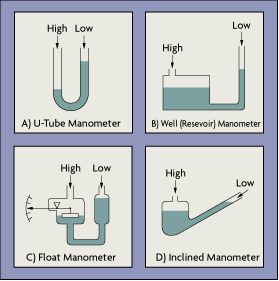
\includegraphics[width=0.5\textwidth]{LiqMano.png}
			\includegraphics[width=0.3\textwidth]{Utube.PNG}
		\end{center}

\end{frame}



\begin{frame}{Liquid Manometer}

\begin{exampleblock}{Features}
               
           \begin{itemize}
           
           		\item Used for Static head and differential pressure  measurement.
 
           		\item Liquid could be Water, Mercury or low vapor pressure oil.
           
          	    \item Suitable for measurement of pressures up to 2 Atm.
           
          \end{itemize}
              
       \end{exampleblock}



\begin{exampleblock}{Advantages}
         
          \begin{itemize}
           
           \item Accurate Measurement. 

           \item Simple construction
           
           \item  Easy to Use.
           
          \end{itemize}
        
       
       \end{exampleblock}
       
       \begin{exampleblock}{Limitations}
          \begin{itemize}
           
           \item Leveling is required before measurement.
           \item Degassing is not possible. 
           
           \item $ LN_{2}$ trap is must to stop liquid vapor to enter the vacuum system. 
           
          \end{itemize}
        
       
       \end{exampleblock}


     


\end{frame}

\begin{frame}{Capacitance Manometer }
\begin{center}
			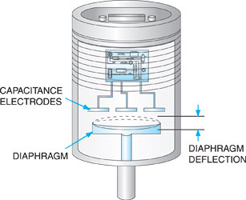
\includegraphics[width=0.5\textwidth]{CapacitanceMano1.png}
			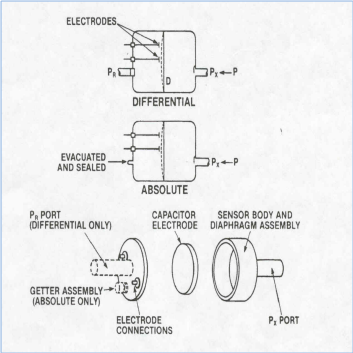
\includegraphics[width=0.5\textwidth]{CapacitanceMano3.png}
		\end{center}

\end{frame}


\begin{frame}{Capacitance Manometer-Working Principle }

       \begin{center}
			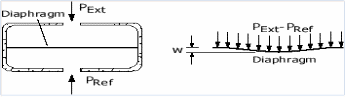
\includegraphics[width=0.5\textwidth]{CapacitanceMano2.png}
			
		\end{center}

			\begin{block}

			   \begin{itemize}

                    \item  Working principle is based on the relationship of parallel plate capacitance $C=\dfrac{\epsilon A}{d}$

					\item   A  thin metal diaphragm separating an unknown pressure from a vacuum, or known pressure. 
 
					\item  The change of  capacitance is a measure of distance between  diaphragm and the fixed electrodes which in turn measure of differentail pressure.
 
					\item   Constructional material may be Inconel and Stainless Steel, allowing the gauge to be used with corrosive gases. 			   		   
			   \end{itemize}
			
			\end{block}

\end{frame}


\begin{frame}{Capacitance Manometer-Signal Processing }
		
		\begin{center}
			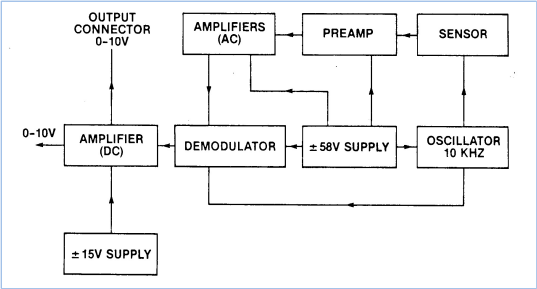
\includegraphics[width=0.8\textwidth]{CapacitanceManoCtrlCkt.png}
		\end{center}

The capacitance change is sensed in an oscillator circuit and converted to a frequency change.
This frequency change, in turn, is converted in the unit to be displayed as the pressure reading.


\end{frame}

\begin{frame}{Capacitance Manometer-Advantage Limitation and Application}

       \begin{exampleblock}{Advantages}
          
          \begin{itemize}
           
           \item Independent of gas or vapor composition.
 
           \item Very high accuracy (0.25 \% to 0.08 \%)
           
           \item Very wide dynamic range (25,000 Torr down to $1 x 10^{-1} $ Torr) .
             
          \end{itemize}
        
       
       \end{exampleblock}
       
       \begin{exampleblock}{Limitations}
          \begin{itemize}
           
           \item Warm up/ Stabilization time after switch on is high compared to many other gauges.
 
           \item Working fluid should be in vapour form at operating temperature.
           
           \item Gauge-head temperature variation is a critical source of error. 
           
           \item Complicated control circuitry.
           
          \end{itemize}
        
       
       \end{exampleblock}



\end{frame}



\begin{frame}{Capacitance Manometer-Application}

     \begin{exampleblock}{Applications}
          
       \begin{itemize}
      		 \item Chemical processes
 			 \item Gas handling manifolds
  			 \item Sputtering
  			 \item Etching systems.
  			 \item Semiconductor manufacturing.
       \end{itemize}                
   
       
       \end{exampleblock}

\end{frame}






\begin{frame}{McLeod Gauge-Construction \& Working }

\begin{exampleblock}{}
          \begin{center}
			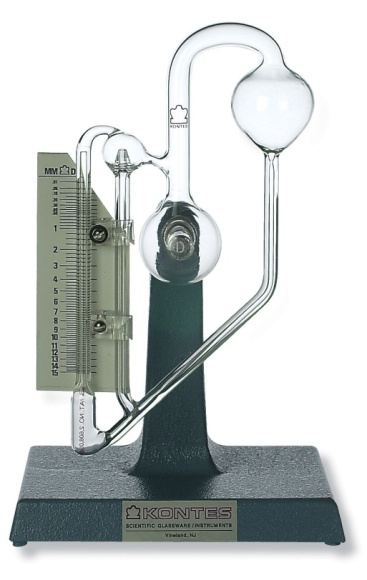
\includegraphics[width=0.4\textwidth]{Macleod.png}
		\end{center}
       \end{exampleblock}

\end{frame}



\begin{frame}{McLeod Gauge-Construction \& Working }

\begin{columns}[t]

\column{0.5\textwidth}
       \begin{exampleblock}{}
          \begin{center}
			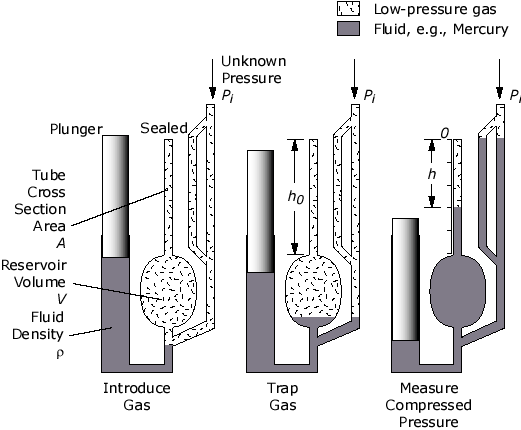
\includegraphics[width=0.95\textwidth]{McLeod.png}
		\end{center}
       \end{exampleblock}
       
    \column{0.5\textwidth}
       \begin{exampleblock}{ }
          From Boyle’s law   $P_{1}V_{1}=P_{2}V_{2} $
Here, $P_{2}=h$ mm column of gas
$V_{2}= \pi r^2 h$ \\
$P_{1}= \dfrac{P_{2}V_{2}}{V_{1}} $\\
= $\pi r^{2}h^{2}/V_{1} $ = $\dfrac{\pi r^{2}}{V_{1}}h^{2}$\\
$P_{1}=K_{g}h^{2}$ mm of Hg \\
 $P_{1}=K_{g}h^{2}$ Torr
       
       \end{exampleblock}   
   
    \end{columns}   



\end{frame}

\begin{frame}{McLeod Gauge-Advantage Limitation }

       \begin{exampleblock}{Advantages}
          \begin{itemize}
           
           \item Reading is very accurate.
     
          \end{itemize}
        
       
       \end{exampleblock}
       
       \begin{exampleblock}{Limitations}
          \begin{itemize}
           
           \item It is bulky and tedious to operate.
           \item Cannot give continuous pressure readings.
           \item Does not give the pressure of non permanent gas.
 			\item $LN_{2}$ trap is must to avoid mercury vapour entering in the vacuum system.
          \end{itemize}
        
       
       \end{exampleblock}


     \begin{exampleblock}{Applications}
                   
           Used as calibration gauge.
                
       \end{exampleblock}

\end{frame}


\begin{frame}{Spinning Rotor Gauge}
				\begin{center}
						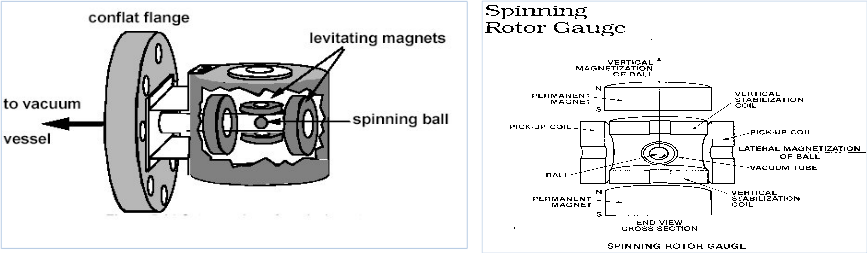
\includegraphics[width=0.6\textwidth]{SpinningRotor.png}
				\end{center}

A ball is magnetically suspended in a small chamber to  eliminate all  sources of friction except the gas friction. The ball is given a rotational velocity of approximately 400 rpm using an electromagnetic coil. Once the speed is constant then accelerating coils are switched off and ball is allowed to coast. The rate of change of rotation is dependent on gas pressure.\\
\begin{center}
$P=\sqrt{\dfrac{8kT}{\pi m}} \dfrac{\pi d \rho}{20 \sigma} \big [\big (\dfrac{\dot{\omega}}{\omega}-RD(\omega))]$
\end{center}




\end{frame}




\begin{frame}{Spinning Rotor Gauge}

	\begin{block}{Advantages of Spinning Rotor Gauge}
      
        \begin{itemize}
          \item     It gives precise vacuum measurements.     
         % \item     It is used to calibrate other gauges.
          \item     It can be used to estimate degassing rate
          
        \end{itemize}
	
	\end{block}

\begin{block}{Disadvantages of Spinning Rotor Gauge}
      
        \begin{itemize}
          \item    It is a very delicate gauge.     
          \item    Any vibration will introduce error in the reading.
          \item    It is expensive.
          \item    Need several minutes for each pressure reading. Hence not very suitable for rapidly varying pressure.
          
        \end{itemize}
	
	\end{block}

\begin{block}{Application}
      
        \begin{itemize}
          \item    Used as calibration gauge.      
          \item    Used in degassing rate  estimation
         
          
        \end{itemize}
	
	\end{block}




\end{frame}

\begin{frame}{Heat Loss in Gas}

	\begin{exampleblock}{}
         		\begin{center}
						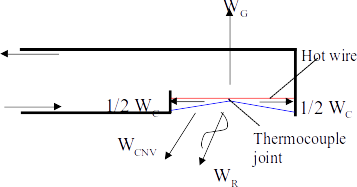
\includegraphics[width=0.4\textwidth]{HeatLoss.png}
						%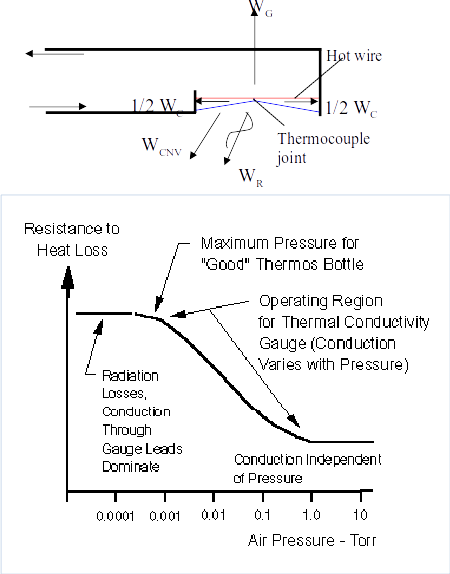
\includegraphics[width=0.9\textwidth]{HeatLossInGas.png}
				\end{center}
       \end{exampleblock}
       
       
 
         		\begin{exampleblock}{ }
         			  Four possible mechanisms to take heat away from sensing element
         			  \begin{itemize}
         			   \item Conduction along sensing element.
         			   \item Conduction through residual gas.
         			   \item Convective \& Radiative heat transfer.
         			   \item Heat taken away by the gas.
         			  \end{itemize}
 						
 				In the pressure range of $10^{-1}$ to $10^{-3} $ Torr heat loss through the gas  is linearly proportional to the pressure. 
       			\end{exampleblock}
            


\end{frame}


\begin{frame}{Heat Loss in Gas}

\begin{columns}[t]
    
      
   \column{0.5\textwidth}
       \begin{exampleblock}{}
         		\begin{center}
						%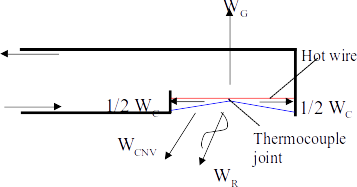
\includegraphics[width=0.9\textwidth]{HeatLoss.png}
						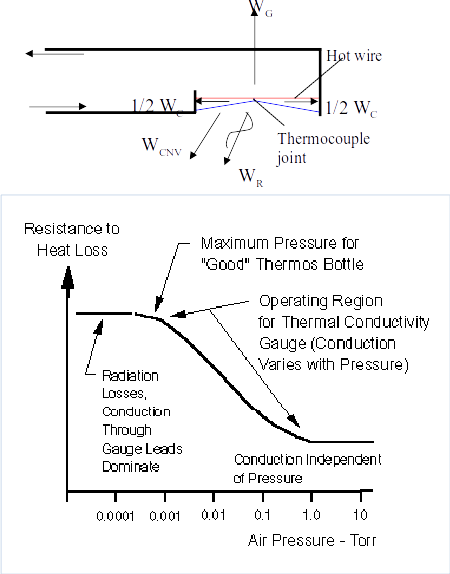
\includegraphics[width=0.9\textwidth]{HeatLossInGas.png}
				\end{center}
       \end{exampleblock}
       
    \column{0.5\textwidth}
       \begin{exampleblock}{ }
          Thermal Conductivity gauge uses this property of the gas to measure the gas pressure in the range 1 to $10^{-3}$ Torr.\\
          There are two types of thermal conductivity gauge 
           \begin{enumerate}
           \item \textbf{Thermocouple Gauge:} This converts the measured temperature of wire into gas pressure.
           \item  \textbf{Pirani Gauge:} This sense the resistance change of the wire and convert it into gas pressure.
           \end{enumerate}
           
       
       \end{exampleblock}   
   
    \end{columns}   




\end{frame}



\begin{frame}{Thermocouple Gauge}
\begin{center}
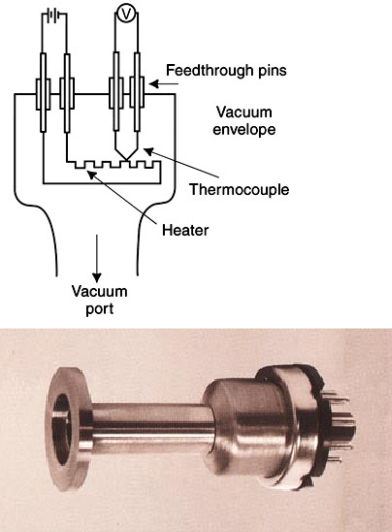
\includegraphics[width=0.5\textwidth]{Thermocouple.png}
\end{center}

	
	

\end{frame}

\begin{frame}{Thermocouple Gauge}

\begin{center}
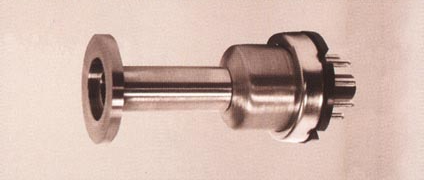
\includegraphics[width=0.3\textwidth]{tc.png}
%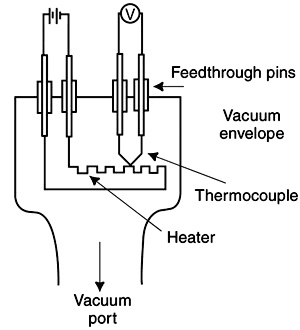
\includegraphics[width=0.2\textwidth]{tc_construction.png}
\end{center}
\begin{block}{Thermocouple Gauge-Salient Points}
      
        \begin{itemize}
          \item A constant current supply feeds the filament.
          \item The gauge measures the voltage of a thermocouple
          \item Spot-welded to a filament exposed to system gas . 
          \item The filament's temperature depends on thermal losses to the gas. At higher pressure the wire will be cooler \& at lower pressure the wire will be hotter.
          \item Since different gases have different thermal conductivities,thermocouple gauge reading is gas dependent.
        \end{itemize}
	
	\end{block}

\end{frame}

\begin{frame}{Thermocouple Gauge}

	\begin{block}{Advantages of Thermocouple Gauge}
      
        \begin{itemize}
          \item    Simple Electronics.
          \item    Most rugged instrument.
          \item    No fear of filament burnout.
          \item    Set points are available.   
        \end{itemize}
	
	\end{block}

\begin{block}{Disadvantages of Thermocouple Gauge}
      
        \begin{itemize}
             
          \item     The gauge stops responding at about $1X 10^{-3}$ Torr because the heat loss through radiation is more significant. 
          \item     The pressure scale is not linear.
          \item     On higher side this gauge does not respond above 2 Torr because above this pressure major heat loss is due to convection .   
                
        \end{itemize}
	
	\end{block}

\end{frame}


\begin{frame}{Pirani Gauge}
\begin{center}
			\includegraphics[width=0.9\textwidth]{Pirani.pdf}
		\end{center}
\end{frame}



\begin{frame}{Pirani Gauge-Working Principle}

\begin{itemize}
\item Two filaments act as resistances in two arms of a Wheatstone bridge. The reference filament is immersed in a fixed gas pressure, while the filament is exposed to the system gas. 
\item Initially the bridge is set  such that the meter reads zero.  A current through the bridge then heats  both filaments.
\item Gas molecules hit the heated filaments and conduct away some of the heat. If the gas pressures (or composition) around the measurement filament is not identical to that around the reference filament, uneven heat is conducted away from both the filament, It results in RESISTANCE CHANGE, and bridge balance gets  upset.
\item This unbalance develops a voltage difference at the meter connections, and current flows  through  it. The meter is calibrated in pressure units. Pirani gauges and their circuitry are typically ten times faster than thermocouple gauges.
\end{itemize}



\end{frame}



\begin{frame}{Advantages and Limitations of Pirani Gauge}
\begin{block}{Advantages of Pirani Gauge}
      
        \begin{itemize}
          \item    It is ten times faster than the thermocouple gauge.
          \item    It is more reliable and accurate than the thermocouple gauge.
            
        \end{itemize}
	
	\end{block}

\begin{block}{Disadvantages of Pirani Gauge}
      
        \begin{itemize}
          
          \item     It is dependent on the gas species.          
        
        \end{itemize}
	
	\end{block}


\begin{block}{Applications}
      
        \begin{itemize}
          
          \item     It is one of the most widely used gauge to measure rough vacuum.  
          \item     In so called full range gauge Pirani gauge measures vacuum in the range 1 to $10^{-3}$ Torr, before cold cathode gauge takes over.        
        
        \end{itemize}
	
	\end{block}

\end{frame}



\begin{frame}{Pirani Gauge-Modifications}
Over the period two major modifications have been taken place in Pirani gauge. They are 
\begin{itemize}
\item \textbf{Convection enhanced Pirani gauge}\\
At high pressure side heat loss due to convection is taken into account.
The convection enhanced Pirani gauge operates by maintaining a sensor wire at some constant temperature.
Monitoring the amount of power required to the keep the sensor wire at a constant temperature, the pressure of the gas can be determined. 


\item \textbf{Micro Pirani gauge}\\
 The Micro Pirani sensor consists of a silicon chip with a heated resistive element forming one surface of a cavity. 
 Due to the geometry of the sensor, convection cannot take place within the cavity and consequently, the sensor is insensitive to the mounting position. 
\end{itemize}

 


\end{frame}

\begin{frame}{Ionization}

\begin{exampleblock}


\begin{enumerate}
		\item Process of formation of positive or negative Ions and free electrons is called \textbf{Ionization}.
\item An atom that loses a single electron is a singly charged positive Ion
\item An atom that loses multiple electrons is a multiply charged positive Ion
\item An atom that that is attached with a single electron is a negative Ion
\item \textbf{Ionization can occur due to \alert{charged particle impact}, heat, radiation.}

		
\end{enumerate}

\end{exampleblock}		


\end{frame}

\begin{frame}{Electron Impact Ionization}

\begin{exampleblock}

\begin{enumerate}
		\item Electric field $ E = \frac{V}{d}$ .
\item If electron travels a distance $\lambda_{e} $  before colliding with a gas atom/molecule (mean free path,  $\approx \num[round-precision=2,round-mode=figures,scientific-notation=true]{0.5e-6}m$ in atmospheric air), it will gain an energy   $ \frac{U \lambda_{e}}{d} = E \lambda_{e} $
\item The minimum energy to remove the weakest bound electron from its normal state in the neutral atom to a distance beyond its sphere of influence is the Ionization Energy
\item Mean free path for electrons is : $ \lambda_{e} = \frac{4\sqrt{2}}{\lambda_{g}} $  and MFP for ions is : $ \lambda_{i} = \frac{\sqrt{2}}{\lambda_{g}} $ 
where $ \lambda_{g} $  is mean free path for gas 

\item Ionization efficiency of Electron
       \begin{itemize}
        \item This is number of ions produced per unit distance per unit gas pressure

        \item This is a function of electron energy

       
        \item The efficiency is maximum at electron energy of about \textbf{100 eV} for most of the gases.

       
       \end{itemize}
       
		
\end{enumerate}

		
\end{exampleblock}

\end{frame}




\begin{frame}{Electron Impact Ionization}

%\begin{exampleblock}
	    \begin{center}
			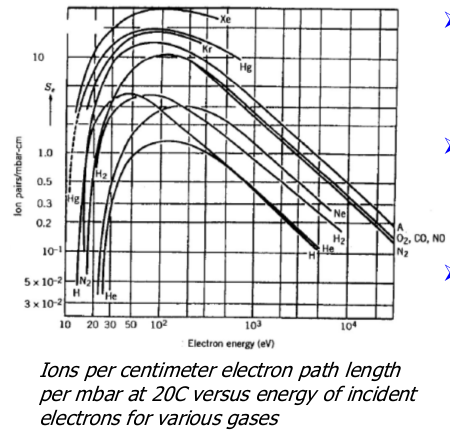
\includegraphics[width=0.3\textwidth]{ElectImpactIonization.png}
		\end{center}	
%\end{exampleblock}

\begin{enumerate}
\item Electron impact ionization rate peaks at electron kinetic energy 50~200 eV for most gases.
\item For hot filament gauges,electrons are emitted thermionically, and accelerated by an electric field.
%Ions per centimeter electron path length per mbar at 20C versus energy of incident electrons for various gases
\item For cold cathode gauges, electrons are initiated by field-emission (or radiations), then trapped/amplified in a cross-field (electric and magnetic fields)
\end {enumerate}



\end{frame}







\begin{frame}{Ionization Gauge}

\begin{columns}[t]
    
      
   \column{0.4\textwidth}
       \begin{exampleblock}{}
          \begin{center}
			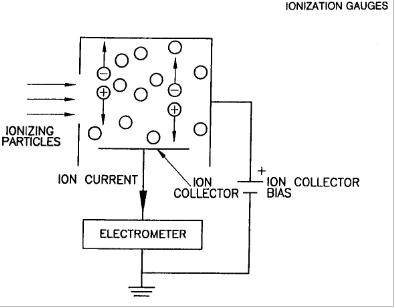
\includegraphics[width=0.9\textwidth]{IonizationGauge.png}
		\end{center}
       \end{exampleblock}
       
    \column{0.6\textwidth}
       \begin{exampleblock}{ }
          \begin{itemize}
            \item PV=nkT     
            \item In Ionization Gauge , neutral gas molecules are ionized and counted , usually by measuring the current.
            \item Ionization normally takes place by electrons, but photons and ions can also be used in special cases.
            \item Ionization Gauges are classified by the method of electron generation.
            \item UHV and EHV region vacuum measurement is solely dependent on Ionization Gauge.
          \end{itemize}
       
       \end{exampleblock}   
   
    \end{columns}   



\end{frame}



\begin{frame}{Ionization Gauge Classification}

		\begin{center}
			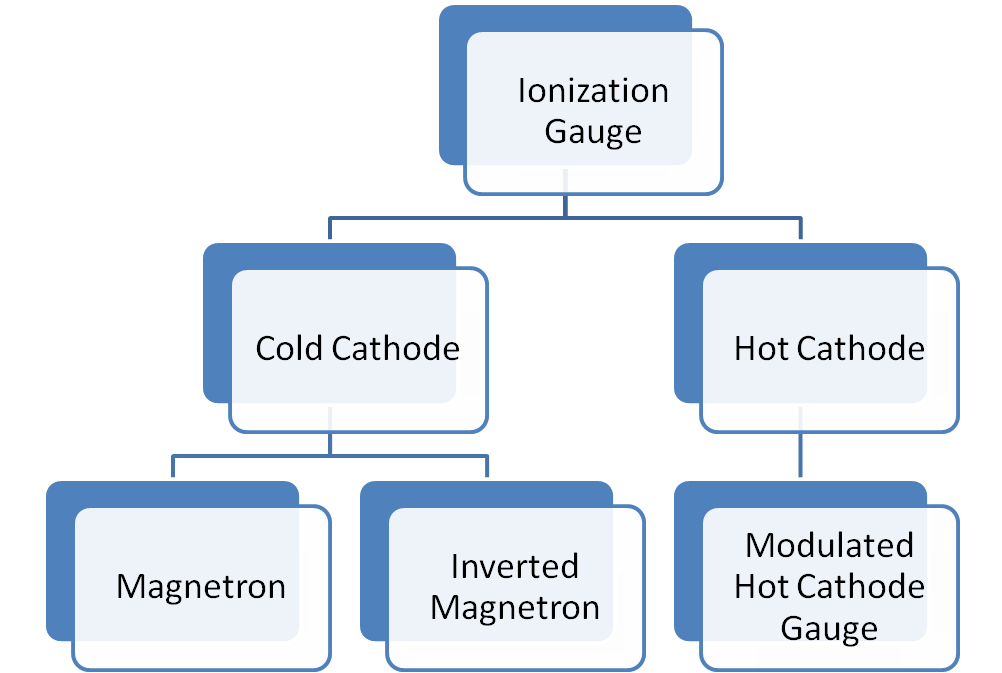
\includegraphics[width=0.9\textwidth]{IG_Classification.png}
		\end{center}


\end{frame}


\begin{frame}{Cold Cathode Gauge}


  \begin{columns}[]
    
      
   \column{0.4\textwidth}
       \begin{exampleblock}{}
         \begin{center}
			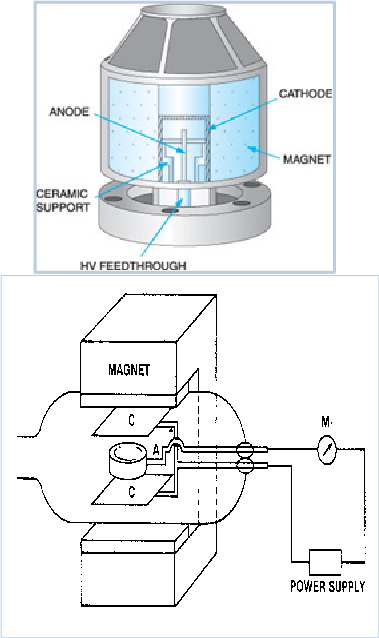
\includegraphics[width=1.0\textwidth]{ColdCathodeGauge.png}
		\end{center}
       \end{exampleblock}
       
    \column{0.6\textwidth}
       \begin{exampleblock}{ }
         
          \begin{itemize}
          		\item Cathode made of Zirconium(Zr) or Thorium(Th). 
          		\item Anode made of stainless steel(SS).
          		\item A permanent magnet.
          		\item High voltage power supply (~2KV).
          		\item Known as \alert{Penning Gauge} after it’s inventor.
          \end{itemize}
       
       \end{exampleblock}   
   
    \end{columns}   

\end{frame}


\begin{frame}{Cold Cathode Gauge}


  \begin{columns}[]
    
      
   \column{0.3\textwidth}
       \begin{exampleblock}{}
         \begin{center}
			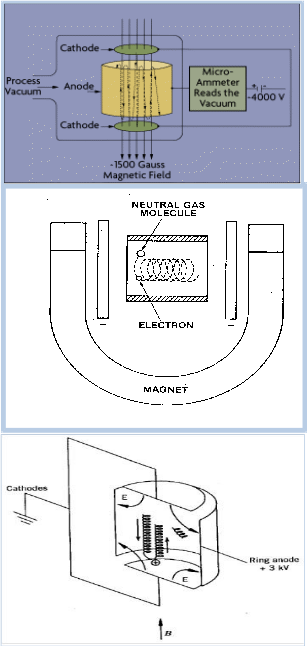
\includegraphics[width=0.95\textwidth]{ColdCathodeGauge1.png}
		\end{center}
       \end{exampleblock}
       
    \column{0.7\textwidth}
       \begin{exampleblock}{ }
          
        \begin{itemize}
          \item Residual electrons ejected from cathode due to \textbf{field emission}. 
          \item Cross magnetic field and electrostatic field forces electrons to take long helical path.
          \item Interaction of electrons with gas molecules causes ionisation.Ions thus formed travel to cathode and gets neutralised.
          \item $I_{+ }= k p^{1.2}$  where $I_{+ }$ = positive ion current , k = constant , p = gas pressure.
          \item Resulting ion current is measured and calibrated in terms of pressure units.
        \end{itemize}
       
       \end{exampleblock}   
   
    \end{columns}   
  
  
  
  
        


\end{frame}



\begin{frame}{Cold Cathode Gauge-Advantages \& Limitations }

       \begin{exampleblock}{Advantages}
          \begin{itemize}
           
           \item Very simple and rugged design.
           \item Ion currents are large enough to be read directly on a sensitive micro ammeter, does not require any calibration, hence no complicated electronics.
           \item Permits measurement in the range $10^{-2}$ Torr to $10^{-5}$ Torr.
     
          \end{itemize}
        
       
       \end{exampleblock}
       
       \begin{exampleblock}{Limitations}
          \begin{itemize}
           
           \item Cold-cathode devices are contaminated more easily and are less stable.
           \item Higher Operating voltage of approximately 2kV.
           \item Accuracy is not as good as hot cathode ionization gauge.
 			\item Ion current is not linearly related to pressure.
 			\item Dependent on gas type.
          \end{itemize}
        
       
       \end{exampleblock}


     

\end{frame}


\begin{frame}{Cold Cathode Gauge-Modifications }

       \begin{exampleblock}{}
         \begin{center}
			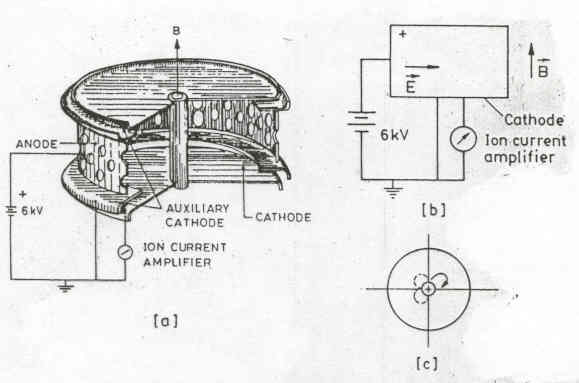
\includegraphics[width=0.5\textwidth]{MagnetronGauge.png}
			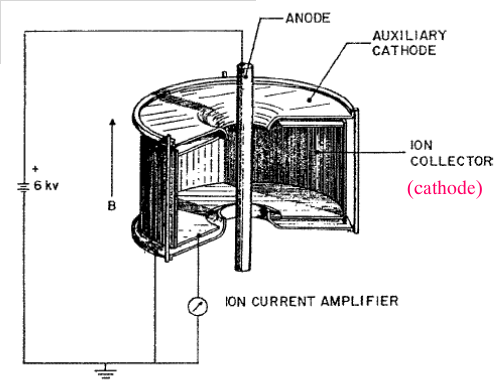
\includegraphics[width=0.5\textwidth]{InvertedMagnetronGauge.png}
		\end{center}
       
       \end{exampleblock}
       
       \begin{exampleblock}{Magnetron and Inverted Magnetron Gauge}
          
        Traditional Penning type cold cathode Ionization gauge design is improved. First improvement is known as magnetron gauge.Next improvement is known as inverted magnetron.\\
        Currently most of the cold cathode gauge is either magnetron or inverted magnetron type.
       
       \end{exampleblock}
       
       
     

\end{frame}



\begin{frame}{Hot Cathode Ionization Gauge-Construction \& Working}

\begin{columns}[t]
    
      
   \column{0.4\textwidth}
       \begin{exampleblock}{}
         \begin{center}
			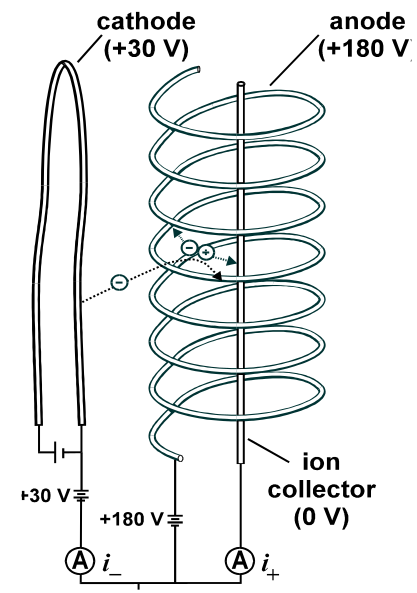
\includegraphics[width=0.7\textwidth]{HCIG.png}
		\end{center}
       \end{exampleblock}
       
    \column{0.6\textwidth}
       \begin{exampleblock}{ }
          \begin{itemize}
          \item Works on the principle of thermo ionic Ionisation of gas molecule. 
          \item It consists of  a hot filament a grid and an ion collector.
          \item The control unit provides power, amplification and metering.
          \item The hot filament supplies ionising electrons.
          \item The grid attracts these electrons.
          \item The Ion collector collects ions, ion current produced is measured in terms of pressure.
          
          \end{itemize}
       
       \end{exampleblock}   
   
    \end{columns}   





\end{frame}




\begin{frame}{Hot Cathode Ionization Gauge Sensitivity}

\begin{columns}[t]
    
      
   \column{0.6\textwidth}
       \begin{exampleblock}{}
         \begin{center}
			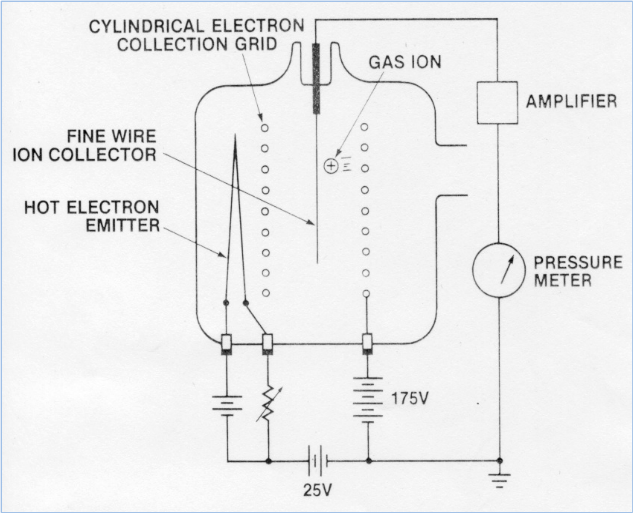
\includegraphics[width=0.9\textwidth]{HotCathodeIonizationGauge.png}
		\end{center}
       \end{exampleblock}
       
    \column{0.3\textwidth}
       \begin{exampleblock}{ }
           $P=\dfrac{1}{S}(\dfrac{I^{+}}{I^{-}}) $ \\
           If  Electron Current $I^{-}$ can be kept constant , then pressure$(P) \propto  I^{+}$ positive ion current.\\
           Control electronics keeps the electron current constant.
       
       \end{exampleblock}   
   
    \end{columns}   





\end{frame}


\begin{frame}{Hot Cathode Ionization Gauge}

\begin{block}{Advantages }
          \begin{itemize}
          \item Reading is very accurate. 
          \item With some modification it can read upto $ 10^{-11} $ Torr
          \end{itemize}
       
       \end{block}  

\begin{block}{Limitations}
          \begin{itemize}
          \item Can not be used at higher pressures more than $1X10^{-3}$ Torr, due to risk of filament burnout. If switched on to atmospheric pressure it will be permanently damaged. 
          \item Do not use this gauge if vacuum interlock is not there , otherwise sudden exposure to atmosphere will permanently damage the hot cathode gauge because of filament burnout. 
          
          \end{itemize}
       
       \end{block}  



\end{frame}

\begin{frame}{Hot Cathode Ionization Gauge}

       \begin{center}
			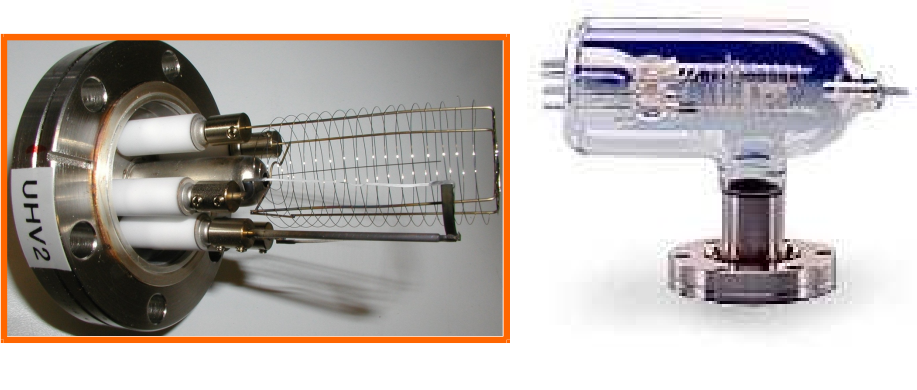
\includegraphics[width=0.75\textwidth]{TwoTypesOfHCIG.png}
		\end{center} 

\end{frame}






\begin{frame}{Hot Cathode Ionization Gauge}


\begin{block}{Limitations}
          \begin{itemize}
          
          \item X-ray limit determines the lower end of the ion gauge range. Low energy X-ray are created when electron strike the grid and when X-rays hit collector, it releases photoelectrons. This causes a constant error signal which is significant at pressures bellow $10^{-10}$ Torr.
          \item At low pressures, in case of glass tube gauges, the Hydrogen permeation through glass is also significant and hence is a source of error.
          \item Calibration depends on the type of gas in the system.
          \end{itemize}
       
       \end{block}  



\end{frame}

\begin{frame}{Hot Cathode Ionization Gauge Soft X Ray Limit}

\begin{center}
			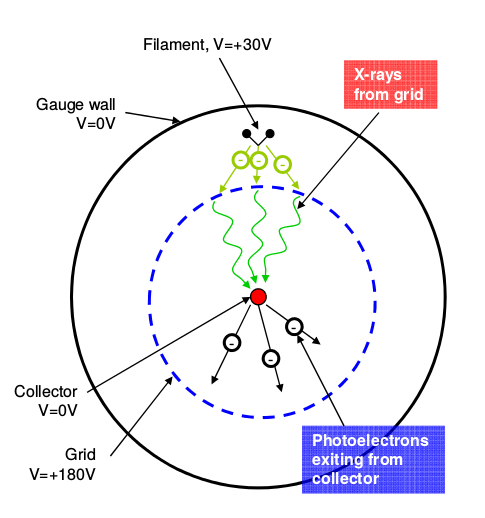
\includegraphics[width=0.25\textwidth]{XrayMechanism.png}
		\end{center} 
		
\begin{block}{ Soft X Ray Mechanism}
          \begin{itemize}
          
          \item Some electrons emitted from the hot cathode impact the grid and produce x-rays.
		  \item Some of the x-rays impact the collector and produce photoelectrons.

			\item The exiting photoelectrons simulate positive ions arriving at the collector. The photoelectron current adds to
the ion current producing an error in the pressure reading.
		
          \end{itemize}
       
       \end{block}  



\end{frame}




		
\begin{frame}{Partial Pr. Measurement}

		\begin{center}
			\includegraphics[width=0.9\textwidth]{PartialPrClassification.pdf}
		\end{center} 


\end{frame}


\begin{frame}{Why Partial Pressure Measurement ?}

		\begin{itemize}
		\item All the gauges discussed earlier measures total gas pressure or density, no information on the gas composition.
        \item Residual gas analyzers are usually incorporated into critical vacuum system as vacuum diagnostic instrument.
        \item In most cases, qualitative mass spectral analysis is sufficient. Sometimes quantitative analysis is need, but
rather difficult.
		\item A RGA measures relative signals verse mass-to-charge ratio (m/e), often in unit of AMU (atomic mass unit).( AMU is defined by C 12 , that is, C 12 has exact 12.0000 AMU )
		\end{itemize}


\end{frame}


\begin{frame}{Components of Residual Gas Analysis System ?}

	\begin{center}
			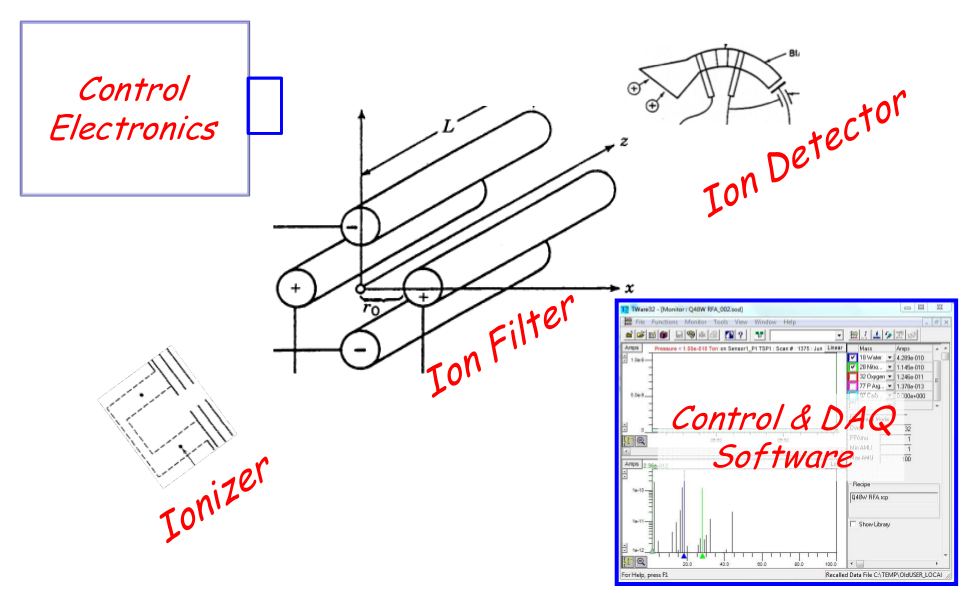
\includegraphics[width=0.9\textwidth]{ResGasAna.png}
		\end{center} 	


\end{frame}

\begin{frame}{Ion Filter}
In general there are three types of ion filters.
	\begin{itemize}
		\item Magnetic Setor(Used mostly in leak checkers, large analytical mass spectrometers)
        \item Quadrupole.(Most widely used in RGAs)
        \item Auto Resonant trap.(Relatively new)
		
		\end{itemize}


\end{frame}


\begin{frame}{Magnetic Sector Ion Filter}

   
  \begin{block}{} 
       \begin{center}
			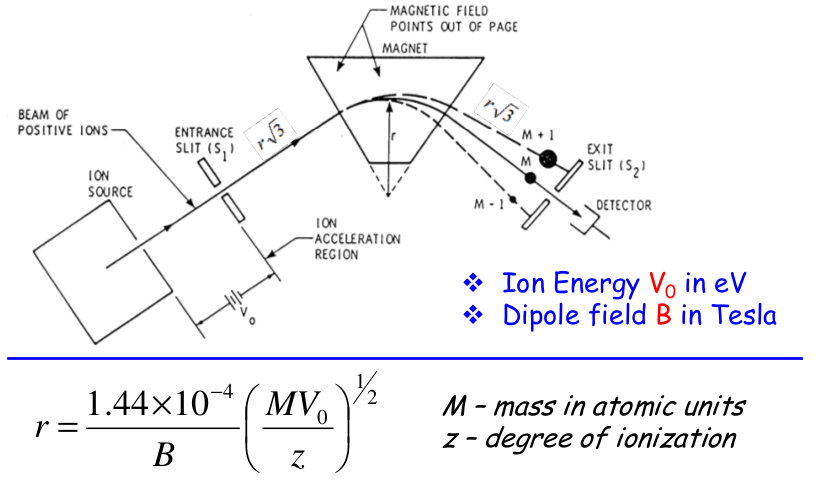
\includegraphics[width=0.7\textwidth]{MagSectIonFilter.png}
		\end{center} 	

\begin{itemize}
 \item If permanent magnet is used then accelerated voltage needs to be changed for scanning.
 \item If electromagnet is used then accelerating voltage may be kept constant and varying magnetic field scanning can be achieved.
\end{itemize}

  \end {block}



\end{frame}


\begin{frame}{Quadrupole Ion Filter}

\begin{block}{} 

		\begin{center}
			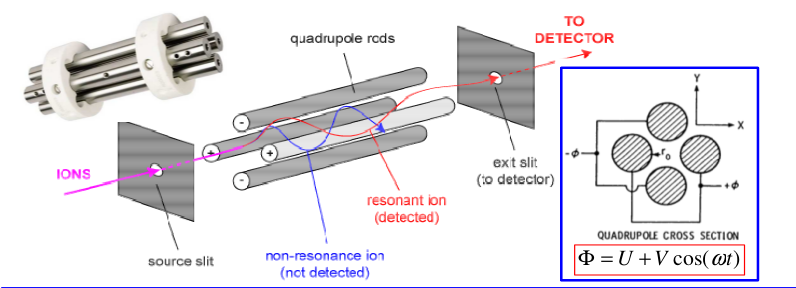
\includegraphics[width=0.6\textwidth]{QuadrupoleIonFilter.png}
		\end{center} 	


\begin{itemize}
 \item Quadrupole Field: $\Phi=\dfrac{(U + V cos \omega t)(x^{2} – y^{2} )}{r_{0}^{2}}$
 \item Ions with certain M/z have stable trajectories to pass through exit aperture at given combination of U and V values.
\end{itemize}

\end {block}

\end{frame}

\begin{frame}{Leak Detection with RGA}

\begin{block}{} 

		\begin{center}
			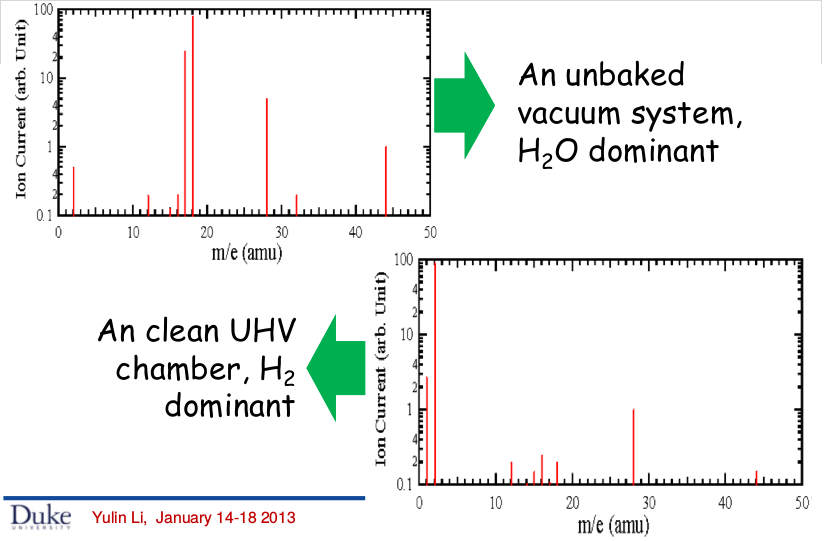
\includegraphics[width=0.8\textwidth]{Unbaked.png}
		\end{center} 	



\end {block}

\end{frame}


\begin{frame}{Leak Detection with RGA}

\begin{block}{} 

		\begin{center}
			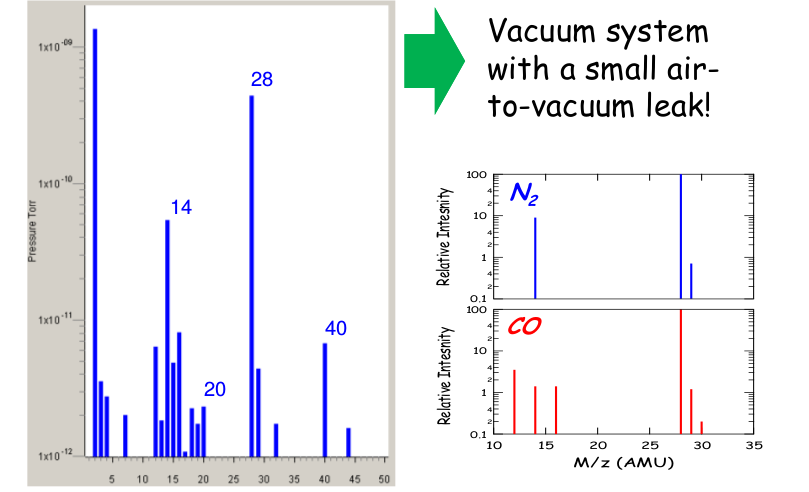
\includegraphics[width=0.8\textwidth]{RealLeak.png}
		\end{center} 	



\end {block}

\end{frame}


\begin{frame}{Selection of Gauges}

When choosing a gauge, consider the following: 
 \begin{itemize}
          \item Cost.
          \item Response time of the gauge.
          \item How the following factor affect it’s performance:
               \begin{itemize}
                 \item Visible or UV radiation.
         		  \item Magnetism.
         		  \item Temperature.
         		  \item Vibration.
         		  \item Corrosive gases
        		\end{itemize}
          \item Accuracy of the measurement. 
          \item Damage caused by switching it on at atmospheric pressure.
        \end{itemize}





\end{frame}


\begin{frame}{Gauge Calibration}


\begin{block}{} 
       \begin{center}
			Under Construction
		\end{center} 	


\end {block}


\end{frame}





\begin{frame}{Gauge Care}


Following care must be taken to improve performance and life of the vacuum gauge.



 \begin{itemize}
          \item Thermal conducivity gauges should be installed away from the heat sources , so that the temperature of the housing never exceeds 288 to 298 K.
          \item Hot cathode ionisation gauges need magnetic shielding when the external field inensity is high.
          \item Due care must be taken to install cold cathode gauge away from the stray magnetic field.
               
          \item Degas gauge before the measurement.
          \item All joints and the and connections between a gauge and the associated vacuum system must be carefully checked for vacuum tightness.
        \end{itemize}





\end{frame}


\begin{frame}{Conclusions}

\begin{itemize}
          \item An 'universal' gauge has not yet been developed for a dynamic range of $10^{15}$. 
          \item Mechanical gauges, in which gas molecules move a liquid or solid diaphragm by hitting it, give absolute pressure measurements unaffected by gas properties. 
          \item Gauges that measure some bulk gas property, such as heat convection, conduction and viscosity, depend on gas composition for their measurements.
               
          \item Gauges for high vacuum (HV) and ultrahigh vacuum (UHV) measurements use charge collection; that is, they ionize residual gas molecules and measure the resulting currents. Although such gauges will ionize vapors as well as permanent gases, differences in ionization potential, ionization cross section, and other parameters, make accurate total pressure measurement of gas mixtures difficult.
         
        \end{itemize}




 



\end{frame}

\begin{frame}{References}

\begin{enumerate}
  \item Cern Accelerator School http://cds.cern.ch/record/923393/files/CERN-2007-003.pdf?version=1
  \item US Particle Accelerator School http://uspas.fnal.gov/materials/13Duke/\\USPASVacuumSession2Gauges.pdf
  
  \item http://www.pfeiffer-vacuum.com/filepool/File/Literature/VTB/Vacuum-Technology-Book-II-Part-2.pdf?referer=2012
  \item http://www.instrumentationtoday.com/
  %\item http://isnap.nd.edu/Lectures/urls/LEYBOLD_FUNDAMENTALS.pdf
\end{enumerate}





\end{frame}

\begin{frame}{Acknowlegements}

\begin{block}{} 

		\begin{center}
			My thanks to \textbf{Indian Vacuum Society} for giving me an opportunity to deliver lecture on vacuum gauges.\\
			My thanks to  Shri S K Gupta \&  Shri A Agarwal. I have learnt vacuum from them. \\
			Thanks to N B V Subhramanyam who helped me preparing these slides.
		\end{center} 	



\end {block}

\begin{block}{} 

		\begin{center}
			\textbf{THANK YOU} for listening.\\
			Send your feedbacks, suggestions, comments and criticisms at arindam@barc.gov.in
		\end{center} 	



\end {block}


\end{frame}





\end{document}


\begin{enumerate}
 \item http://cds.cern.ch/record/923393/files/CERN-2007-003.pdf?version=1
 \item http://uspas.fnal.gov/materials/13Duke/USPASVacuumSession2Gauges.pdf
 \item http://www.pfeiffer-vacuum.com/filepool/File/Literature/VTB/Vacuum-Technology-Book-II-Part-2.pdf?referer=2012
 \item http://isnap.nd.edu/Lectures/urls/LEYBOLD_FUNDAMENTALS.pdf
\end{enumerate}